%==============================================================================
% SOEN 6481 - Systems Requirements Specification
% Delivery #1 - Vision Document (Rational Unified Process)
% Project: Healthy Living  |  Product: NourishU (web based application)
% Author: Sohana Mahmud
%==============================================================================
\documentclass[11pt,a4paper]{article}

\usepackage[utf8]{inputenc}
\usepackage[T1]{fontenc}
\usepackage{lmodern}
\usepackage[margin=1in]{geometry}
\usepackage{graphicx}
\usepackage[table]{xcolor}
\usepackage{booktabs}
\usepackage{array}
\usepackage{tabularx}
\usepackage{longtable}
\usepackage{enumitem}
\usepackage{fancyhdr}
\usepackage{titlesec}
\usepackage{parskip}
\usepackage{caption}
\usepackage{tikz}
\usetikzlibrary{shapes.geometric, arrows.meta, positioning, fit, backgrounds}
\usepackage[hidelinks]{hyperref}

%------------------------------------------------------------------------------
% Colors
%------------------------------------------------------------------------------
\definecolor{concordiagold}{RGB}{146,29,45}   % Concordia maroon
\definecolor{nourishgreen}{RGB}{34,110,72}
\definecolor{lightgreen}{RGB}{233,244,238}
\definecolor{headergray}{RGB}{90,90,90}
\definecolor{tablehead}{RGB}{34,110,72}
\definecolor{tablealt}{RGB}{240,247,243}
\definecolor{bandblue}{RGB}{240,244,247}
\definecolor{bandext}{RGB}{251,243,244}

%------------------------------------------------------------------------------
% Section formatting
%------------------------------------------------------------------------------
\titleformat{\section}{\Large\bfseries\color{nourishgreen}}{\thesection.}{0.5em}{}
\titleformat{\subsection}{\large\bfseries\color{concordiagold}}{\thesubsection}{0.5em}{}
\titleformat{\subsubsection}{\normalsize\bfseries\color{headergray}}{\thesubsubsection}{0.5em}{}
\titlespacing*{\section}{0pt}{14pt}{6pt}

%------------------------------------------------------------------------------
% Header and footer
%------------------------------------------------------------------------------
\pagestyle{fancy}
\fancyhf{}
\renewcommand{\headrulewidth}{0.6pt}
\renewcommand{\headrule}{\hbox to\headwidth{\color{nourishgreen}\leaders\hrule height \headrulewidth\hfill}}
\fancyhead[L]{\footnotesize\textbf{\color{nourishgreen}NourishU} \textcolor{headergray}{Vision Document}}
\fancyhead[R]{\footnotesize\textcolor{headergray}{Concordia University | SOEN 6481}}
\fancyfoot[C]{\footnotesize\thepage}
\fancyfoot[R]{\footnotesize\textcolor{headergray}{CS \& SE Dept.}}

\newcolumntype{Y}{>{\raggedright\arraybackslash}X}
\renewcommand{\arraystretch}{1.35}

% Project links (edit if your repository name differs)
\newcommand{\githublink}{https://github.com/SohanaMahmud/SOEN6481-Healthy-Living-SRS}

%==============================================================================
\begin{document}

%------------------------------------------------------------------------------
% TITLE PAGE
%------------------------------------------------------------------------------
\begin{titlepage}
\centering
\vspace*{0.5cm}

{\color{concordiagold}\rule{\textwidth}{2pt}}\\[0.4cm]
{\Large\bfseries GINA CODY School of Engineering and Computer Science}\\[0.2cm]
{\large Department of Computer Science and Software Engineering}\\[0.2cm]
{\large Concordia University}\\[0.3cm]
{\large\bfseries SOEN 6481 Systems Requirements Specification}\\[0.2cm]
{\color{concordiagold}\rule{\textwidth}{2pt}}\\[1.2cm]

{\Huge\bfseries\color{nourishgreen} NourishU}\\[0.4cm]
{\LARGE\itshape Healthy Living Made Simple and Affordable}\\[0.3cm]
{\large A web based application}\\[1.0cm]

{\Large\bfseries Vision Document}\\[0.3cm]
{\large Delivery \#1}\\[0.3cm]
{\large Rational Unified Process (RUP)}\\[1.6cm]

\begin{tabular}{rl}
\textbf{Student Name:} & Sohana Mahmud \\[0.3cm]
\textbf{Student ID:} & 40271073\\[0.3cm]
\textbf{Course:} & SOEN 6481, Summer 2026 \\[0.3cm]
\textbf{Professor:}& Dr.\ Morales \\[0.3cm]
\textbf{Date:} & July 12, 2026\\[0.3cm]
\textbf{Version:} & 1.1 \\
\end{tabular}

\vspace{0.9cm}
{\footnotesize\textbf{Project repository:} \url{\githublink}}

\vfill
{\footnotesize\color{headergray} Prepared in the role of Requirements Engineer.\\
This document addresses both the problem and solution domains at a high level of abstraction.}
\end{titlepage}

%------------------------------------------------------------------------------
% REVISION HISTORY + TOC
%------------------------------------------------------------------------------
\section*{Revision History}
\renewcommand{\arraystretch}{1.3}
\begin{tabularx}{\textwidth}{l l l Y}
\toprule
\rowcolor{tablehead}\textcolor{white}{\textbf{Version}} & \textcolor{white}{\textbf{Date}} & \textcolor{white}{\textbf{Author}} & \textcolor{white}{\textbf{Description}} \\
\midrule
1.0 & July 10, 2026 & Sohana Mahmud & Initial Vision Document for the Healthy Living Project (Delivery \#1). \\
1.1 & \today & Sohana Mahmud & Scope refined to a web based application. Added a high level block diagram and a User Personal Profile feature. Features aligned with profile driven dietary, religious, cuisine, calorie, and budget factors for breakfast, lunch, and dinner across weekdays and weekends. \\
\bottomrule
\end{tabularx}

\vspace{0.8cm}
{\color{nourishgreen}\hrule}
\newpage
\tableofcontents
{\color{nourishgreen}\hrule}
\newpage

%==============================================================================
% 1. INTRODUCTION
%==============================================================================
\section{Introduction}

The purpose of this Vision Document is to outline the goals, stakeholders, high-level needs, and product features for \textbf{NourishU}, a web-based application created as part of the Healthy Living project. NourishU assists university students in organizing balanced weekly meals, adhering to simple recipes, and managing a restricted food budget. The document outlines the problem to be addressed and presents the planning of balanced weekly meals, following simple recipes, and managing limited requirements and use cases in subsequent deliverables.

Many students, particularly those planning to live independently for the first time, find it challenging to maintain a healthy diet while balancing a constrained budget, a hectic class schedule, and limited culinary abilities. Students possess personal and cultural needs that generic tools often overlook, including halal requirements, food allergies, and dietary restrictions, as well as a preference for familiar cuisines, such as meal plans for breakfast, lunch, and dinner that take into account each student's dietary and religious requirements, cuisine preferences, calorie goals, and budget, with plans that can vary between weekdays and weekends.

This document acts as a common reference point that aligns the project team, the sponsor, and future reviewers on the objectives and purpose of NourishU. It is designed to develop as feedback is received from the sponsor and subsequent deliverables; the content here may undergo revisions, with each change being documented in the project version control repository.

\subsection{References}

\begin{itemize}[leftmargin=1.5em, itemsep=2pt]
    \item SOEN 6481 Delivery \#1 assignment description, Healthy Living project, by Dr.\ Morales.
    \item SOEN 6481 Delivery \#1 grading rubric, CS \& SE Department, Concordia University.
    \item SOEN 6481 Vision Document template, CS \& SE Department, Concordia University.
    \item SOEN 6481 course lectures on Requirements Engineering, Requirements Elicitation, and the Vision Document and Product Features.
    \item Concordia University Academic Code of Conduct.
    \item P. Kruchten, \textit{The Rational Unified Process: An Introduction}, Addison Wesley.
    \item Canada's Food Guide, Health Canada, used as a reference for nutrition guidance principles.
    \item Project repository (GitHub): \url{\githublink}
\end{itemize}

%==============================================================================
% 2. POSITIONING
%==============================================================================
\newpage
\section{Positioning}

\subsection{Problem Statement}

\begin{tabularx}{\textwidth}{>{\bfseries\raggedright\arraybackslash}p{0.30\textwidth} Y}
\toprule
\rowcolor{tablehead}\textcolor{white}{\textbf{Element}} & \textcolor{white}{\textbf{Description}} \\
\midrule
The problem of & eating in a healthy and balanced way that also respects personal, religious, and cultural food needs while staying within a limited budget \\
\rowcolor{tablealt}
affects & university students, in particular those who live independently; cook for themselves; follow requirements such as halal or have allergies and food restrictions; and manage tight food budgets and busy schedules \\
the impact of which is & poor nutrition and skipped meals, difficulty finding meals that fit religious, allergy, and cuisine needs, overspending and repeated last-minute takeout, wasted time deciding what to eat, and added stress that can affect academic performance and wellbeing \\
\rowcolor{tablealt}
a successful solution would be & a single, easy-to-use web application that plans balanced weekly meals for breakfast, lunch, and dinner around each student's budget, calorie target, dietary and religious needs, allergies, and cuisine preferences, and suggests simple recipes, with plans that adapt for weekdays and weekends \\
\bottomrule
\end{tabularx}

\subsection{Product Position Statement}

\begin{tabularx}{\textwidth}{>{\bfseries\raggedright\arraybackslash}p{0.22\textwidth} Y}
\toprule
\rowcolor{tablehead}\textcolor{white}{\textbf{Element}} & \textcolor{white}{\textbf{Description}} \\
\midrule
For & university students who need to eat healthily on a limited budget \\
\rowcolor{tablealt}
Who & want weekly meal plans and recipes that fit their calorie target, budget, religious and dietary needs such as halal, their allergies and restrictions, and their preferred cuisines, without spending hours planning \\
NourishU & is a web based healthy meal planning application \\
\rowcolor{tablealt}
That & builds personalized weekly plans for breakfast, lunch, and dinner within a set budget and calorie target, respects dietary, religious, allergy, and cuisine preferences; and recommends simple recipes, with separate weekday and weekend plans \\
Unlike & generic recipe websites, standalone calorie counters, and manual spreadsheets that ignore budget, religious and cultural food needs, and cuisine variety \\
\rowcolor{tablealt}
Our product & connects nutrition, calories, cost, culture, and personal restrictions into one student focused web experience that is affordable and easy to use \\
\bottomrule
\end{tabularx}

%==============================================================================
% 3. STAKEHOLDER DESCRIPTIONS
%==============================================================================
\section{Stakeholder Descriptions}

This section identifies the people and groups who have an interest in NourishU. It separates non user stakeholders, who influence or are affected by the product without operating it directly, from the users who interact with the system.

\subsection{Stakeholder Summary}

\begin{tabularx}{\textwidth}{>{\bfseries\raggedright\arraybackslash}p{0.24\textwidth} Y Y}
\toprule
\rowcolor{tablehead}\textcolor{white}{\textbf{Name}} & \textcolor{white}{\textbf{Description}} & \textcolor{white}{\textbf{Responsibilities}} \\
\midrule
Sponsor (Course Instructor) & Dr.\ Morales, who sponsors the project and represents the interests of the funding organization during the course. & Sets the vision and priorities, approves scope and features, provides feedback during class and office hours, and validates that the product meets the intended goals. \\
\rowcolor{tablealt}
Project Team (Requirements Engineer and Developers) & The individuals responsible for eliciting requirements, and for designing, building, testing, and maintaining NourishU. & Elicit and specify requirements, design the architecture, implement and test features, and keep the documentation and repository up to date. \\
Nutrition Advisor & A registered dietitian or nutrition expert who advises on healthy eating guidance. & Reviews nutrition rules, calorie targets, and recipe content for accuracy, and helps ensure meal plans follow accepted dietary guidelines. \\
\rowcolor{tablealt}
University Student Services & Campus wellbeing, residence, and food services groups interested in student health and affordability. & Provide context on student needs, and may promote the app within campus services in the future. \\
Grocery and Data Providers & Third party sources of grocery pricing, product, and nutrition data. & Supply reliable price and product information used for budgeting and grocery features. \\
\rowcolor{tablealt}
Marketing and Outreach & The group responsible for positioning and promoting NourishU to students. & Communicate the value of the product, gather user feedback, and support adoption on campus. \\
\bottomrule
\end{tabularx}

\subsection{User Summary}

\begin{tabularx}{\textwidth}{>{\bfseries\raggedright\arraybackslash}p{0.20\textwidth} Y Y >{\raggedright\arraybackslash}p{0.16\textwidth}}
\toprule
\rowcolor{tablehead}\textcolor{white}{\textbf{Name}} & \textcolor{white}{\textbf{Description}} & \textcolor{white}{\textbf{Responsibilities}} & \textcolor{white}{\textbf{Stakeholder}} \\
\midrule
Student (Primary End User) & The central persona for whom the app is built. A university student who manages personal meals, budget, and daily intake. & Sets up a profile with budget, calorie target, dietary, religious, allergy, and cuisine preferences, generates and follows weekly meal plans, views recipes, and rates them. & Self represented \\
\rowcolor{tablealt}
System Administrator (Admin) & The technical user responsible for backend maintenance, security, and the overall health of the application. & Manages accounts, roles, and permissions, monitors performance and security, applies updates, and maintains backups. & Project Team \\
Content Moderator / Content Manager & A user responsible for overseeing the recipe and nutrition database to ensure quality and safety. & Reviews, approves, edits, and publishes recipe and nutrition content, verifies halal and allergen labels, and removes inaccurate or unsafe material. & Nutrition Advisor \\
\rowcolor{tablealt}
Support Specialist & The user who handles customer service and addresses technical or functional issues raised by students. & Responds to support requests, troubleshoots issues, escalates defects to the team, and maintains help resources. & Project Team \\
\bottomrule
\end{tabularx}

\subsection{User Environment}

\begin{itemize}[leftmargin=1.5em, itemsep=3pt]
    \item The primary users are a group of students who generally handle their own meals, either for themselves or occasionally for a shared household of two to five individuals. The system is anticipated to cater to a small pilot group of students initially, with the capacity to expand to several thousand active users as adoption increases on campus.
    \item Students engage with NourishU in brief, regular sessions. Common cycles consist of planning meals for the week at the beginning, conducting brief daily reviews of the meals for breakfast, lunch, and dinner, and making occasional adjustments to preferences.
    \item NourishU is a web-based application that can be accessed through a standard web browser on a laptop, desktop, or the browser of a phone or tablet. No separate application installation is necessary.
    \item Weekday and weekend routines differ. Students often want quicker, simpler meals on busy class days and more flexible or elaborate meals on weekends, so plans can differ for weekdays and weekends.
    \item Users possess a diverse array of cooking skills and varying levels of technical proficiency. The interface should be straightforward, necessitating minimal training, and must be operational in English at the time of launch, with the option to incorporate French and additional languages subsequently, considering the bilingual environment of Montreal.
    \item The system relies on external grocery pricing and nutrition data, and it must protect personal information such as dietary preferences, religious and health-related notes, allergies, and budget records in line with app health-related expectations.
\end{itemize}

\subsection{Key Stakeholder or User Needs}

\begin{longtable}{>{\raggedright\arraybackslash}p{0.20\textwidth} >{\raggedright\arraybackslash}p{0.09\textwidth} >{\raggedright\arraybackslash}p{0.22\textwidth} >{\raggedright\arraybackslash}p{0.19\textwidth} >{\raggedright\arraybackslash}p{0.24\textwidth}}
\toprule
\rowcolor{tablehead}\textcolor{white}{\textbf{Need}} & \textcolor{white}{\textbf{Priority}} & \textcolor{white}{\textbf{Concerns}} & \textcolor{white}{\textbf{Current Solution}} & \textcolor{white}{\textbf{Proposed Solution}} \\
\midrule
\endhead
Budget aware meal planning & High & Students overspend and cannot see the cost of a week of meals in advance. & Manual budgeting or none. & Weekly meal plans generated within a set budget, with a clear running cost estimate. \\
\rowcolor{tablealt}
Calorie and balanced nutrition & High & Hard to know if meals are balanced or meet a calorie target. & Guessing or scattered advice. & Plans and recipes aligned with nutrition guidance and a chosen calorie target. \\
Halal and religious dietary needs & High & Generic tools ignore religious food requirements such as halal. & Manual checking of ingredients. & Preference settings that keep all suggested meals within the selected religious and dietary rules. \\
\rowcolor{tablealt}
Allergies and food restrictions & High & Suggested meals may contain allergens or restricted items. & Reading labels one by one. & Personalized plans that exclude declared allergens and restrictions and flag them clearly. \\
Cuisine preference and variety & Medium & Plans feel repetitive or unfamiliar to the student's culture. & Searching separate recipe sites. & Cuisine selection such as Chinese or South Indian, kept healthy and balanced. \\
\rowcolor{tablealt}
Weekday and weekend flexibility & Medium & The same plan does not fit busy weekdays and freer weekends. & Ad hoc daily decisions. & Separate weekday and weekend plans for breakfast, lunch, and dinner. \\
Simple, low cost recipes & High & Limited time and skill lead to unhealthy choices. & Random recipe searches. & A curated recipe library filtered by budget, time, skill, and preferences. \\
\rowcolor{tablealt}
Efficient grocery shopping & Medium & Shopping is disorganized, leading to forgotten items and waste. & Handwritten lists. & Auto generated grocery lists based on the chosen weekly plan. \\
\bottomrule
\end{longtable}

%==============================================================================
% 4. PRODUCT OVERVIEW
%==============================================================================
\section{Product Overview}

\subsection{Product Perspective}

NourishU is a self-contained web application designed for students, supported by a shared cloud database. Users can access it via a modern web browser without the need for any additional software installation. The system consolidates weekly meal planning, recipes, calorie and budget tracking, and grocery lists, which are currently scattered across various unrelated tools, into a single account for ease of use.

The product engages with a limited selection of external services, including grocery pricing and nutrition data sources, as well as an optional email notification service. These integrations are separated by clearly defined interfaces, ensuring that the core experience remains functional even if an external service is temporarily inaccessible. The high-level block diagram below illustrates the primary components of NourishU, structured into a presentation layer, an application layer comprising core modules, and a data layer, alongside the users and external services that engage with the system.

\vspace{0.3cm}
\begin{figure}[h]
\centering
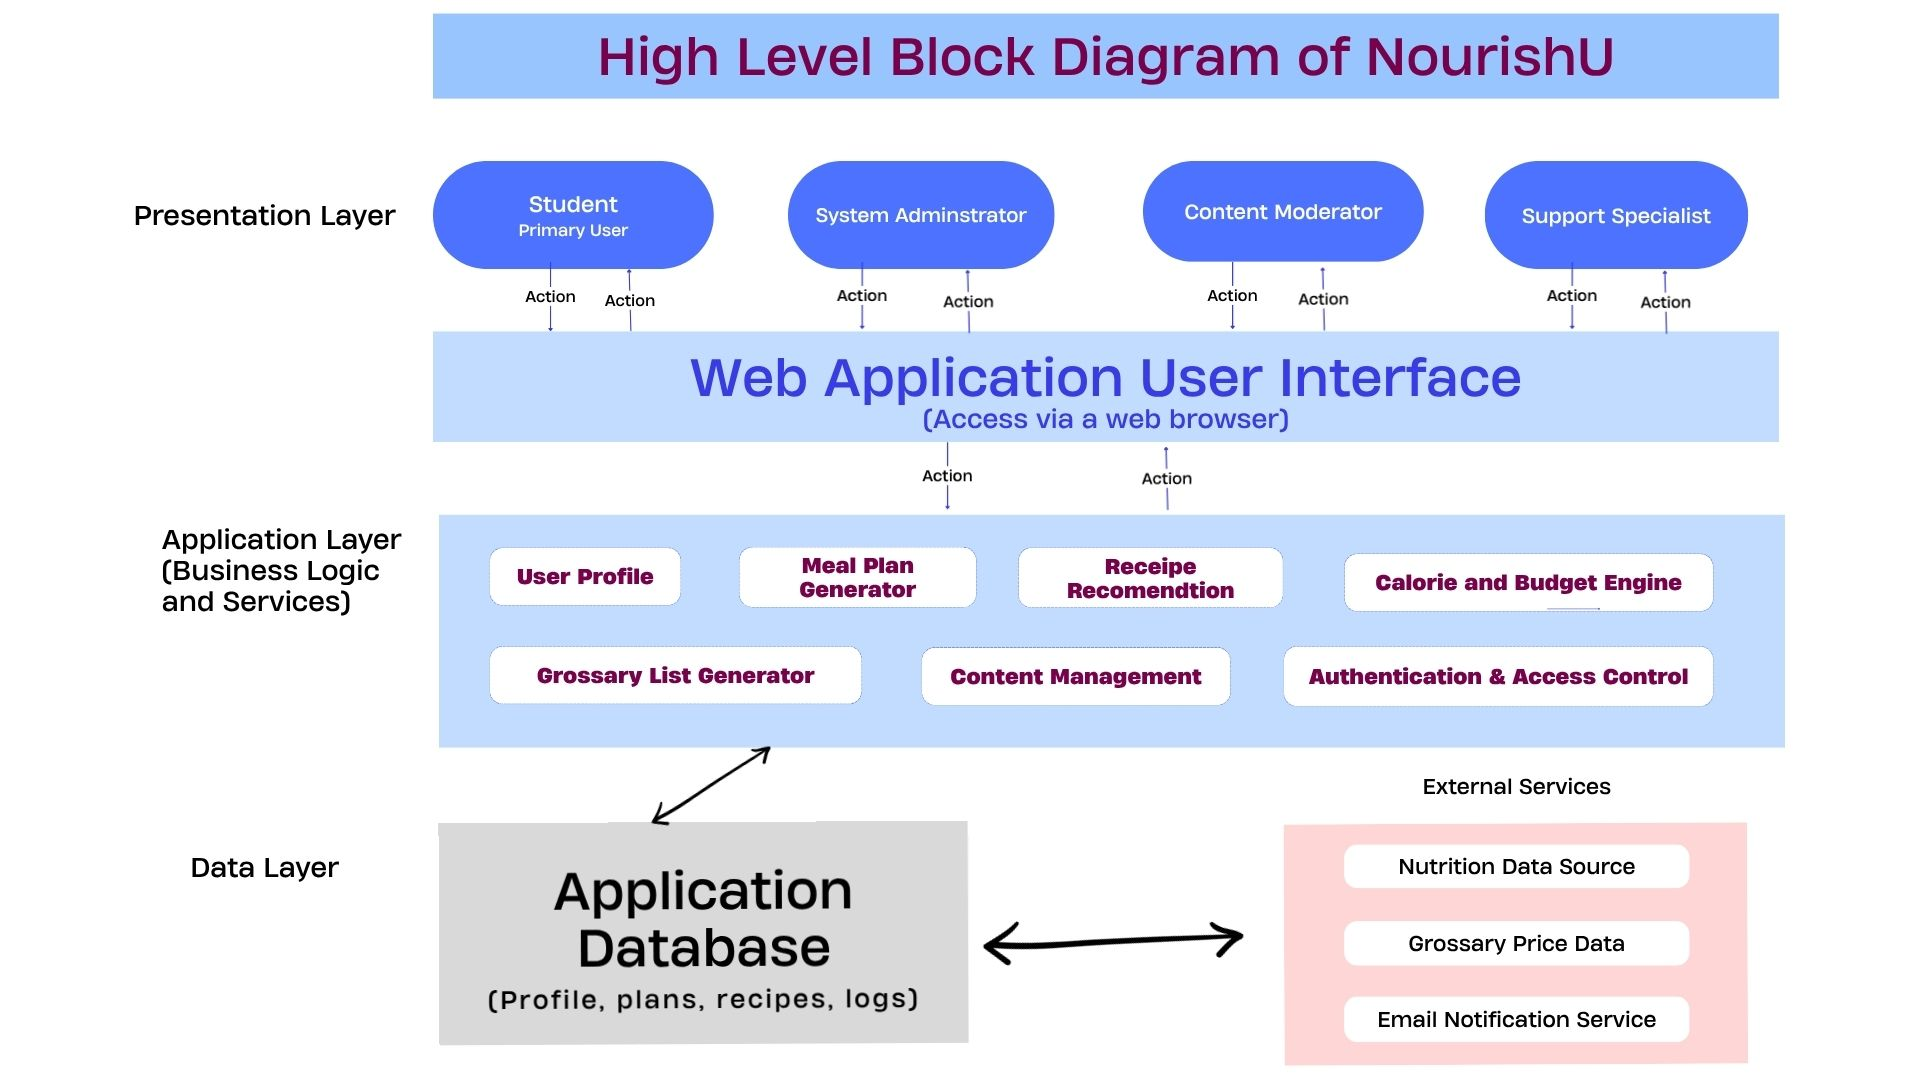
\includegraphics[width=1.1\textwidth]{block_diagram.jpg}
\caption*{\footnotesize \textbf{Figure 1.} High level block diagram of NourishU.}
\end{figure}

\subsection{Assumptions and Dependencies}

\begin{tabularx}{\textwidth}{Y Y}
\toprule
\rowcolor{tablehead}\textcolor{white}{\textbf{Assumptions}} & \textcolor{white}{\textbf{Dependencies}} \\
\midrule
Students have access to a modern web browser with internet access. & The web client depends on current browser versions being maintained. \\
\rowcolor{tablealt}
Reliable grocery pricing and nutrition data can be obtained from external providers or a maintained internal dataset. & Budget, calorie, and grocery features depend on the availability and accuracy of these data sources, with a fallback to cached or default data when a source is unavailable. \\
Students are willing to enter a budget, calorie target, and preferences such as halal, allergies, and cuisine to receive personalized plans. & Personalization quality depends on the information students provide and keep up to date. \\
\rowcolor{tablealt}
Hosting resources such as cloud servers, storage, and a domain will be available for deployment. & Deployment and performance depend on the chosen cloud hosting provider and network availability. \\
Nutrition and halal or allergen content is reviewed by a qualified advisor before publication. & Content quality depends on timely review by the Nutrition Advisor and Content Moderator. \\
\rowcolor{tablealt}
Applicable privacy expectations for personal, religious, and health related data will be respected. & Compliance depends on secure storage, authentication services, and adherence to data protection practices. \\
\bottomrule
\end{tabularx}

%==============================================================================
% 5. PRODUCT FEATURES
%==============================================================================
\section{Product Features}

This section lists the high level features of NourishU. Detailed behavior will be elaborated as use cases and requirements in later deliverables.

\subsection{User Personal Profile}
Every student has a personal profile that serves as the foundation of the entire experience. The profile contains personal details, food preferences, and various likes and dislikes. It includes dietary and religious requirements such as halal or vegetarian options, allergies, and restricted ingredients. Additionally, it outlines the weekly budget, daily calorie target, and any special conditions the student wishes to note, such as diabetes or a low sodium requirement. The student establishes this setup once and can modify it at any time, with every meal plan and recipe suggestion being generated from this profile, ensuring that the results consistently align with the individual student.

\subsection{Weekly Meal Planning}
Based on the student's profile, NourishU generates a personalized weekly meal plan covering breakfast, lunch, and dinner for each day. Plans can differ between weekdays and weekends so that busy class days get quicker, simpler meals and weekends allow more flexibility. Students can view the full week at a glance and regenerate or swap individual meals.

\subsection{Budget-Aware Planning}
Each plan is built to fit within the weekly food budget in the student's profile. As the plan is created, the system shows a running estimate of the total cost, so students can see before shopping whether the week fits their budget, and it can adjust suggestions to stay within the limit.

\subsection{Calorie and Nutrition Awareness}
Using the calorie target from the profile, the system builds plans that aim to meet it while keeping meals balanced. Clear nutrition summaries are shown for each meal and for the overall day and week, aligned with recognized dietary guidance.

\subsection{Halal and Religious Dietary Preferences}
The profile can record religious dietary requirements such as halal. Once set, every suggested meal and recipe respects these rules, and content is labeled so students can trust the suggestions.

\subsection{Allergy and Food Restriction Management}
The system uses the allergies and food restrictions declared in the profile to exclude those ingredients from all plans and recipes, and it clearly flags any allergens present in related items.

\subsection{Cuisine Preference Selection}
Students can choose preferred cuisines such as Chinese, South Indian, and others in their profile. The system prioritizes recipes from those cuisines while keeping the meals healthy and balanced, giving students familiar food that still meets nutrition goals.

\subsection{Recipe Library and Suggestions}
Students have the opportunity to explore and search through a carefully selected library of simple, affordable recipes. The system suggests recipes tailored to individual profiles, taking into account factors such as budget, calorie goals, preparation time, skill level, dietary and religious requirements, allergies, and preferred cuisine. Each recipe features a list of ingredients, detailed step-by-step instructions, calorie information, and an estimated cost.

\subsection{Smart Grocery List}
From the selected weekly plan, the system automatically builds a grocery list of exactly what the student needs to purchase, grouped by category such as produce, dairy, and pantry items, so students can shop efficiently and reduce waste.

\subsection{Meal and Budget Tracking}
Students can optionally log the meals they actually ate and the money they spent, and view simple summaries of calories and spending over the week to understand their habits and adjust future plans.

\subsection{Ratings and Feedback}
Students can rate recipes and provide feedback. This helps improve recommendations and gives content managers signals about which recipes work well.

\subsection{Content Management and Moderation}
Content Moderators can review, edit, approve, and publish recipe and nutrition content through a dedicated interface, and verify halal and allergen labels, keeping the database accurate and safe.

\subsection{User and Access Management}
The System Administrator manages accounts, roles, and permissions through role based access control, ensuring each type of user reaches only the features appropriate to their role.

\subsection{Help and Support}
Students can access help resources and submit support requests. Support Specialists can respond, track, and escalate issues, supported by an in app help center.

%==============================================================================
% 6. OTHER PRODUCT REQUIREMENTS
%==============================================================================
\section{Other Product Requirements}

\begin{longtable}{>{\bfseries\raggedright\arraybackslash}p{0.24\textwidth} >{\raggedright\arraybackslash}p{0.75\textwidth}}
\toprule
\rowcolor{tablehead}\textcolor{white}{\textbf{Requirement}} & \textcolor{white}{\textbf{Description}} \\
\midrule
\endhead
Usability & The interface must be simple and require little training. Core tasks, such as generating a weekly meal plan or grocery list, should be completable in a few steps, and the design should be accessible to users with varying technical skill. \\
\rowcolor{tablealt}
Performance & The system should respond to common actions quickly, typically presenting content within a few seconds under normal load, so that planning feels smooth. \\
Availability & The service should be available around the clock, with any scheduled maintenance communicated to users in advance and kept as short as possible. \\
\rowcolor{tablealt}
Scalability & The architecture should scale from a small pilot group to several thousand active users without redesign. \\
Security and Privacy & Personal, religious, dietary, allergy, and budget data must be protected. The system requires secure authentication, encrypted storage of sensitive data, and access to personal information only by the owner or authorized roles. \\
\rowcolor{tablealt}
Reliability and Fault Tolerance & The system should keep working and preserve data integrity during partial failures, with regular backups and graceful handling of unavailable external services. \\
Compatibility & The web application must work on current major web browsers such as Chrome, Firefox, Edge, and Safari, and be responsive on common screen sizes. \\
\rowcolor{tablealt}
Accessibility & The product should follow accessibility good practices so that students with disabilities can use core features. \\
Localization & English is supported at launch, with the design allowing French and other languages to be added later. \\
\rowcolor{tablealt}
Standards and Compliance & The system should follow applicable data protection expectations and web security good practices. \\
Documentation and Support & User guidance, help content, and support channels must be available and kept current. \\
\bottomrule
\end{longtable}

%==============================================================================
% 7. APPENDIX
%==============================================================================
\newpage

\section{Appendix}

\subsection{Activity Logs}

The table below records the time spent on each section of this Vision Document, as required by Task 0. Replace the placeholder dates with the actual dates on which you worked on each section.

\begin{tabularx}{\textwidth}{>{\raggedright\arraybackslash}p{0.16\textwidth} Y >{\raggedright\arraybackslash}p{0.18\textwidth}}
\toprule
\rowcolor{tablehead}\textcolor{white}{\textbf{Date}} & \textcolor{white}{\textbf{Section}} & \textcolor{white}{\textbf{Time Spent}} \\
\midrule
\mbox{[09/07/2026]} & Basic Requirement Analysis, study references, draft Introduction and References & 4.0 h \\
\rowcolor{tablealt}
\mbox{[09/07/2026]} & Prepare draft and Positioning & 3.0 h \\
\mbox{[10/07/2026]} & Stakeholder Descriptions & 2.5 h \\
\rowcolor{tablealt}
\mbox{[12/07/2026]} & Product Overview and Block Diagram & 4.0 h \\
\mbox{[10/07/2026]} & Product Features & 3.0 h \\
\rowcolor{tablealt}
\mbox{[11/07/2026]} & Other Product Requirements & 2.0 h \\
\mbox{[12/07/2026]} & Appendix and Final Review and Overall Update & 4.0 h \\
\midrule
\multicolumn{2}{r}{\textbf{Total}} & \textbf{22.5 h} \\
\bottomrule
\end{tabularx}

\subsection{Glossary}

\begin{tabularx}{\textwidth}{>{\bfseries\raggedright\arraybackslash}p{0.26\textwidth} Y}
\toprule
\rowcolor{tablehead}\textcolor{white}{\textbf{Term}} & \textcolor{white}{\textbf{Definition}} \\
\midrule
NourishU & The name of the Healthy Living product described in this document. \\
\rowcolor{tablealt}
RUP & Rational Unified Process, the software development framework whose Vision Document format is followed here. \\
User Profile & The personal record for each student that stores choices, dietary and religious needs, allergies, budget, calorie target, and special conditions, and that drives all meal and recipe suggestions. \\
\rowcolor{tablealt}
Meal Plan & A schedule of meals for a period, usually a week, covering breakfast, lunch, and dinner, generated by the system based on the student's profile, budget, calories, and preferences. \\
Halal & Food prepared and permitted according to Islamic dietary law. A preference students can set so all suggestions comply. \\
\rowcolor{tablealt}
Dietary Restriction & A limitation on what a student can or will eat, for religious, medical, allergy, or personal reasons. \\
Allergen & An ingredient that can cause an allergic reaction, which the system excludes and flags based on the student's declared allergies. \\
\rowcolor{tablealt}
Cuisine Preference & A student's preferred style of food, such as Chinese or South Indian, used to guide recipe suggestions while keeping meals healthy. \\
Calorie Target & The daily energy intake a student aims for, used to build balanced plans. \\
\rowcolor{tablealt}
Grocery List & A categorized list of items to buy, generated from the weekly meal plan. \\
Role Based Access Control (RBAC) & A method of restricting system access based on the role assigned to each user. \\
\rowcolor{tablealt}
Stakeholder & Any person or group with an interest in the project who is not necessarily a direct user of the system. \\
Sponsor & The party who owns the vision and priorities for the product, represented in this course by the instructor. \\
\bottomrule
\end{tabularx}

\subsection{Tools Used and Generative AI Acknowledgment}

The manuscript for this document was prepared using LaTeX in Overleaf, and the source is maintained under version control in the project GitHub repository (\url{\githublink}). Generative AI tools were used to assist with brain-storming, initial drafting, formatting, and organizing the content according to the Vision Document template. All requirement, decisions, stakeholder analysis, and features presented here reflect my own understanding of the Healthy Living project, and I have analyzed, designed, documented, reviewed, and verified the content. This use of tools follows the course syllabus guidelines on generative AI and the Concordia University Academic Code of Conduct.

\medskip
{\footnotesize\itshape }

\end{document}
